\documentclass[]{article}
\usepackage{lmodern}
\usepackage{amssymb,amsmath}
\usepackage{ifxetex,ifluatex}
\usepackage{fixltx2e} % provides \textsubscript
\ifnum 0\ifxetex 1\fi\ifluatex 1\fi=0 % if pdftex
  \usepackage[T1]{fontenc}
  \usepackage[utf8]{inputenc}
\else % if luatex or xelatex
  \ifxetex
    \usepackage{mathspec}
  \else
    \usepackage{fontspec}
  \fi
  \defaultfontfeatures{Ligatures=TeX,Scale=MatchLowercase}
\fi
% use upquote if available, for straight quotes in verbatim environments
\IfFileExists{upquote.sty}{\usepackage{upquote}}{}
% use microtype if available
\IfFileExists{microtype.sty}{%
\usepackage{microtype}
\UseMicrotypeSet[protrusion]{basicmath} % disable protrusion for tt fonts
}{}
\usepackage[margin=1in]{geometry}
\usepackage{hyperref}
\hypersetup{unicode=true,
            pdftitle={Problem sets - GTA guide},
            pdfborder={0 0 0},
            breaklinks=true}
\urlstyle{same}  % don't use monospace font for urls
\usepackage{graphicx,grffile}
\makeatletter
\def\maxwidth{\ifdim\Gin@nat@width>\linewidth\linewidth\else\Gin@nat@width\fi}
\def\maxheight{\ifdim\Gin@nat@height>\textheight\textheight\else\Gin@nat@height\fi}
\makeatother
% Scale images if necessary, so that they will not overflow the page
% margins by default, and it is still possible to overwrite the defaults
% using explicit options in \includegraphics[width, height, ...]{}
\setkeys{Gin}{width=\maxwidth,height=\maxheight,keepaspectratio}
\IfFileExists{parskip.sty}{%
\usepackage{parskip}
}{% else
\setlength{\parindent}{0pt}
\setlength{\parskip}{6pt plus 2pt minus 1pt}
}
\setlength{\emergencystretch}{3em}  % prevent overfull lines
\providecommand{\tightlist}{%
  \setlength{\itemsep}{0pt}\setlength{\parskip}{0pt}}
\setcounter{secnumdepth}{0}
% Redefines (sub)paragraphs to behave more like sections
\ifx\paragraph\undefined\else
\let\oldparagraph\paragraph
\renewcommand{\paragraph}[1]{\oldparagraph{#1}\mbox{}}
\fi
\ifx\subparagraph\undefined\else
\let\oldsubparagraph\subparagraph
\renewcommand{\subparagraph}[1]{\oldsubparagraph{#1}\mbox{}}
\fi

%%% Use protect on footnotes to avoid problems with footnotes in titles
\let\rmarkdownfootnote\footnote%
\def\footnote{\protect\rmarkdownfootnote}

%%% Change title format to be more compact
\usepackage{titling}

% Create subtitle command for use in maketitle
\providecommand{\subtitle}[1]{
  \posttitle{
    \begin{center}\large#1\end{center}
    }
}

\setlength{\droptitle}{-2em}

  \title{Problem sets - GTA guide}
    \pretitle{\vspace{\droptitle}\centering\huge}
  \posttitle{\par}
    \author{}
    \preauthor{}\postauthor{}
    \date{}
    \predate{}\postdate{}
  

\begin{document}
\maketitle

\hypertarget{ps1}{%
\subsection*{First problem set: Mathematical approaches, economic
models, revision and warm-up}\label{ps1}}
\addcontentsline{toc}{subsection}{First problem set: Mathematical
approaches, economic models, revision and warm-up}

\textcolor{Grey}{We will cover key parts of this problem set in the first tutorial (as well as part of the second problem set). However, you should aim to be able to do and understand all of the material on the assigned problem sets.}

\emph{Goals of this problem set:}

\begin{itemize}
\item
  Re-acquaintance with mathematical approaches to Economics (e.g.,
  simultaneous equations, graphing functions)
\item
  Revising the supply and demand model and its implications, applying
  this to real-world problems, considering \emph{empirical} approaces
\item
  Understanding the logic of `difficult' multiple choice questions
  (\emph{assessment} tips)
\item
  Discussing and writing a coherent response to applied Economics
  questions
\end{itemize}

\hypertarget{problem-1-drawing-demand-and-supply-computation}{%
\subsubsection*{Problem 1: drawing demand and supply,
computation}\label{problem-1-drawing-demand-and-supply-computation}}
\addcontentsline{toc}{subsubsection}{Problem 1: drawing demand and
supply, computation}

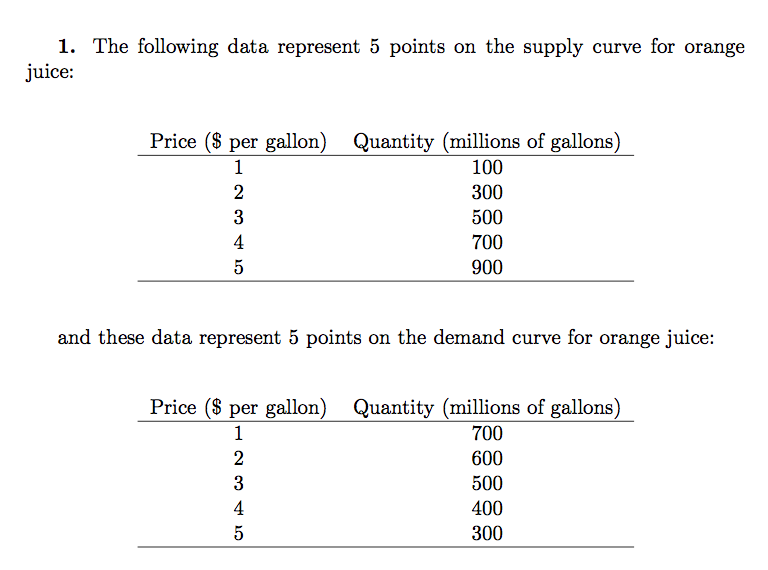
\includegraphics{ns_prob1.png}

\begin{center}\rule{0.5\linewidth}{\linethickness}\end{center}

\hypertarget{a-graph-the-points-of-these-supply-and-demand-curves-for-orange-juice.-be-sure-to-put-price-on-the-vertical-axis-and-quantity-on-the-horizontal-axis.}{%
\subsubsection*{1.1.A: Graph the points of these supply and demand
curves for orange juice. Be sure to put price on the vertical axis and
quantity on the horizontal
axis.}\label{a-graph-the-points-of-these-supply-and-demand-curves-for-orange-juice.-be-sure-to-put-price-on-the-vertical-axis-and-quantity-on-the-horizontal-axis.}}
\addcontentsline{toc}{subsubsection}{1.1.A: Graph the points of these
supply and demand curves for orange juice. Be sure to put price on the
vertical axis and quantity on the horizontal axis.}

(If this is tedious, just graph three points for each).

\textbf{Ans:}

\begin{figure}

{\centering 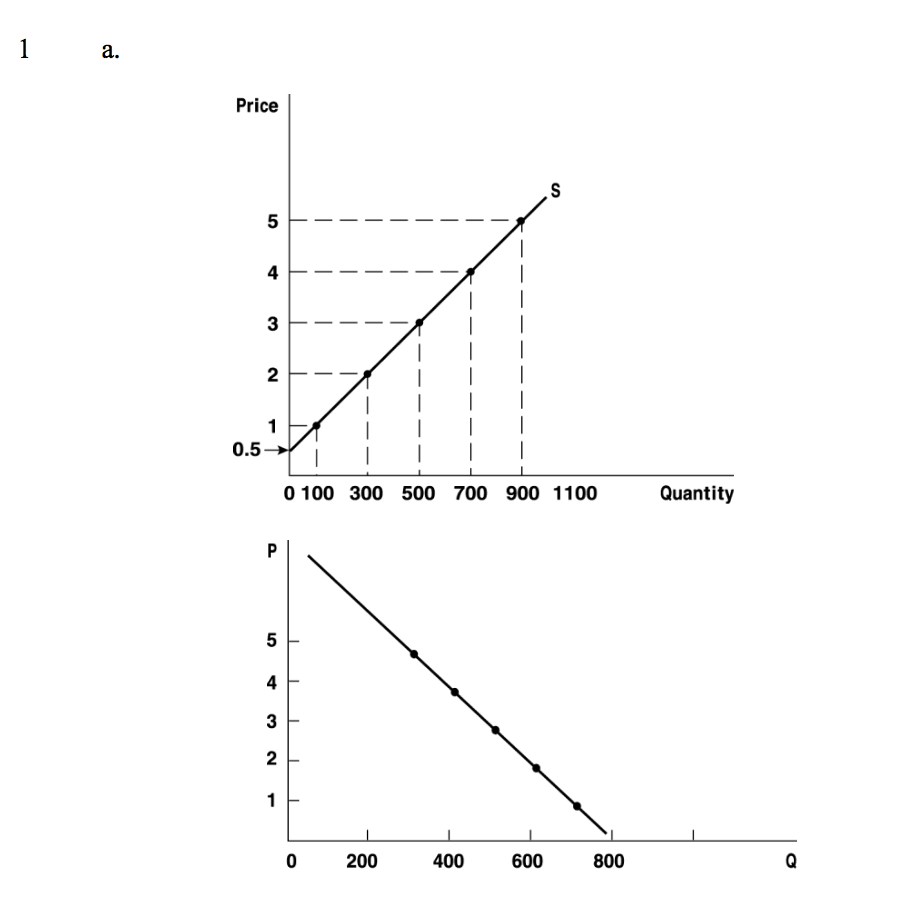
\includegraphics[width=0.9\linewidth]{ns1a_ans} 

}

\end{figure}

\textcolor{red}{GTA's:} Ten minutes, i.e., minutes 5-15 of of tutorial,
perhaps (after introducing yourself etc).

Really try to get the students involved in doing this\ldots{} call on
them, ask questions, bring them up, have them do it on their desks or
show their answers in pairs

1.1.a-b should be very easy for most. However, there are likely some
students who are math-challenged and actually do need to think about
this carefully. There are also (unfortunately) a cohort of students who
have not really taken Economics before!

Explain the axes briefly, and what each point means (ask students
first). Graph a few points, connect the lines, have students comment on
the slope and whether it `makes sense'.

Try to get them to make a correct statement about why `demand curves
slope down' (at a higher price, fewer consumers are willing to buy, and
consumers willing to buy fewer units, because at a higher price, they
can do better by buying other things with that money) and why `supply
curves slope up'.

Be careful to make a distinction between `Demand curves' and `Quantity
demanded'. \emph{Avoid} the use of ambiguous language like `demand
increases'.

Ask them to consider how would one find `points on a supply curve'
versus `points on a demand curve'; remember that in the real-world by
simply observing prices and quantities we don't know whether we are
seeing shifts in a demand curve, shifts in a supply curve, or both.

\textbf{1.1.B: Do these points lie along two straight lines? If so,
figure out the precise algebraic equation of these lines. (Hint: If the
points do lie on straight lines, you need only consider two points on
each of them to calculate the lines.) }

\emph{Yes, they do. The `rise over run' between any two points is the
same.}

\textcolor{gray}{E.g., for supply, when price rises from 1 to 2,  quantity supplied rises from 100 to 300, for a 'rise over run' of 200/1=200.
OK, as we plot price on the vertical axis, we could say that the "rise" is the rise in price of 2-1=1 and the "run" is the rise in quantity supplied or 300-100=200, for a 'rise over run' of 1/200.}

\textcolor{gray}{For any other pair of points on this supply curve this is the same; e.g as price rises from 3 to 5, $Q_s$ rises from 500 to 900, for a 'rise over run' of $5-3/900-500 = 2/400=1/200$}

\textcolor{gray}{For the demand curve we could make similar calculations but the slopes will be negative.}

\emph{Now to figure out the algebraic equation\ldots{}}

\begin{itemize}
\item
  (Recall GCSE maths formula for straight line: \(y=mx+b\))
\item
  This is a linear function \(P = a+bQ\) (when we get to demand, we
  allow \(b\) to be negative)
\end{itemize}

\emph{Essentially repeating the above `rise over run'
calculation'\ldots{}}

\begin{itemize}
\tightlist
\item
  For supply, increase P by 1 and Q increases by 200. (See diagram)

  \begin{itemize}
  \tightlist
  \item
    i.e, for \(\Delta P = 1\), \(\Delta Q = 200\)
  \item
    \ldots{} implying that if price were to increase by 1, firms would
    be willing to provide 200 more units in total
  \end{itemize}
\end{itemize}

\textcolor{gray}{Doing this more carefully ... if we have any two points, $x_1,y_1$ and $x_2,y_2$ we can compute the slope $m= rac{y_2-y_1}{x_2-x_1}$, again 'rise over run'.}

\textcolor{gray}{Take any two points on the supply curve (the table above), and compute this to get the slope.}

\textcolor{gray}{E.g., $(P_1,Q_1)$ = $(1,100)$ and $(P_2,Q_2)$=$(2,300)$.  The slope is thus $rac{(300-100)}{(2-1)}=200.$ as stated above. However, this is the slope of $Q$ in $P$. Confusingly, although economists usually consider how $Q$ changes in $P$ along supply (or demand curves), our convention is to plot $P$ on the vertical axis an $Q$ on the horizontal. So, when drawing the slope, remember to keep this straight. If the slope of Q in P is 200, the slope of P in Q is actually the inverse of this, namely $1/200$. (Check: $\frac{P_2-P_1}/{Q2-Q1}=1/200$). Also note that a slope of $1/200$ would look almost flat, so it's better to make the quantity axis in units of 100, so you can do a slope of 1/2 (vertical increase of 1 units for each 2 units of horizontal increase).}

\begin{itemize}
\tightlist
\item
  Thus \(\frac{\Delta P}{\Delta Q} = \frac{1}{200}\)

  \begin{itemize}
  \tightlist
  \item
    We know the slope \(b=\frac{1}{200}\)
  \item
    \(\rightarrow P = a + \frac{q}{200}\)
  \end{itemize}
\end{itemize}

\emph{What about the intercept \(a\)?} Just plug some value into the
formula and solve for this. - at \(P=2\), \(Q=300\) -
\(\rightarrow 2 = a + \frac{300}{200} = a + \frac{3}{2}\) - so
\(a = \frac{1}{2}\) - Thus the equation is
\(P = \frac{1}{2} + \frac{Q_s}{200}\) - or \(Q_s=200P-100\)

\footnote{Check: does this equation describe the graph? Is it intuitive? Supply upward-sloping in price. Intercept: $P>1/2$ necessary for a positive quantity supplied.}

For demand, increase P by 1 and Q declines by 100.

\begin{itemize}
\tightlist
\item
  Solves similarly to above:

  \begin{itemize}
  \tightlist
  \item
    \(\rightarrow\) \(P=8-\frac{Q_d}{100}\) or \(Q_d=800-100p\)
  \end{itemize}
\end{itemize}

\textcolor{red}{GTA's:} Go slowly, but not too slowly, with this algebra
for the first few computations. Remember that some students may have
completely forgotten all maths!

\begin{center}\rule{0.5\linewidth}{\linethickness}\end{center}

\textbf{1.1.C: Use your solutions from part b to calculate the ``excess
demand'' for orange juice if the (imposed) market price is zero}

\begin{itemize}
\tightlist
\item
  Note that for the supply curve, quantity supplied is never negative --
  below a certain price, it will just be zero.

  \begin{itemize}
  \tightlist
  \item
    Consider: (why) does this make sense?
  \end{itemize}
\end{itemize}

*More technically, firms choose among their feasible `production sets',
which must be non-negative.

\textbf{Ans:}

\begin{itemize}
\tightlist
\item
  Draw these functions on the same graph to aid intuition
\end{itemize}

\textcolor{red}{GTA's:} Do draw this on the board, this time on the same
axes (supply and demand curves together) \ldots{} or add one to the
other, already on the board.

\begin{itemize}
\tightlist
\item
  \(Q_s(P)=200P-100\), at \(P=0\), \(Q_s = -100\)

  \begin{itemize}
  \tightlist
  \item
    we must not forget that we actually mean \(Q_s(p)=max(0,200P-100)\),
    so \(Q_s(0) = 0\)
  \end{itemize}
\end{itemize}

\textcolor{red}{GTA's:} Let's explain at this point what the ``max'' and
``min'' functions mean. Give a few examples.

\begin{itemize}
\tightlist
\item
  \(Q_d(P)=800-100P\) \(\rightarrow\) \(Q_d(0)=800\)
\item
  \(\rightarrow\) Excess demand at \(P = 0\) is
  \(Q_d(0)-Q_s(0)=800-0 = 800\).
\end{itemize}

\emph{Consider: does this make sense? If the government declared `orange
juice must be free' and imposed no subsidies, would you expect there to
be excess demand?}

\textcolor{red}{GTA's:} The students are likely to find this difficult,
especially the `max' thing. Practice how to explain this in advance so
you don't get tongue-tied.

\begin{center}\rule{0.5\linewidth}{\linethickness}\end{center}

\textbf{1.1.D: Use your solutions from part b to calculate the ``excess
supply'' for orange juice if the orange juice price is \$6 per gallon.}

\begin{itemize}
\tightlist
\item
  We will skip this in tutorial because it's basically the same task as
  part c
\end{itemize}

Ans: Excess supply at \(P=6\) is 900

\textcolor{red}{GTA's:} Please skip this part.

\hypertarget{mcqs-from-previous-exams-slightly-adjusted-these-were-some-of-the-hardest-ones-they-are-not-all-so-difficult}{%
\subsubsection*{MCQs from previous exams, slightly adjusted (these were
some of the hardest ones, they are not all so
difficult)}\label{mcqs-from-previous-exams-slightly-adjusted-these-were-some-of-the-hardest-ones-they-are-not-all-so-difficult}}
\addcontentsline{toc}{subsubsection}{MCQs from previous exams, slightly
adjusted (these were some of the hardest ones, they are not all so
difficult)}

\textcolor{red}{GTA's:} Do the other MCQ's first (further below). Cover
these only briefly {[}5-10 minutes{]}, if time permits, focusing on the
logic/strategy of answering MCQ's.

\textbf{MCQ2 True or False: One example of microdata is a set of over 5
million observations of income, hours worked, and demographic
information from over 1 million households' tax returns over five
years.}

\bigskip

\textbf{Answer:}

True. Microdata refers to the level of the unit of observation; the
economic decision-maker, such as an individual or household, rather than
an aggregation, such as an entire country or market. 65\% got this one
right.

\textcolor{gray}{Note – this was covered in the mini-lecture ‘Empirical microeconomics/econometrics’ as well as in the text. Again, this is a ‘challenge question’; if you read carefully, and read the suggested applications and additional readings, you should be able to get most of these questions. However, I don’t expect everyone will get these right, so I will limit the number of such questions so that you can still get a good mark without knowing these.
I want you to have more than just a ‘textbook theoretical’ understanding. Understanding how data is used in business, economic analysis, and policy, will be very important in your career!}

\bigskip

\textbf{MCQ3 True or false: It is valid to plot observed prices and
quantities traded in a market and fit a line through them to estimate a
market demand curve.}

\textbf{Answer:} False. "If we plot prices and quantities traded in a
market, we are be observing the interaction of shifts in supply and
demand curve, so it is difficult to estimate either curve without
further assumptions. About 30\% got this one right.

\textcolor{gray}{Again, this is a challenge question. Remember: I will ask some questions where the answer is not ‘common-sense’ answer that someone who has not taken Economics would give. And this is what you should want: if you study and engage, you should understand more after taking this module than you did when you started it!}

\bigskip

\textbf{MCQ4 (Choose all that are correct): The slope of the production
possibility frontier}

\begin{itemize}
\item
  \begin{enumerate}
  \def\labelenumi{\alph{enumi}.}
  \tightlist
  \item
    shows how inputs must be changed to keep them fully employed.
  \end{enumerate}
\item
  \begin{enumerate}
  \def\labelenumi{\alph{enumi}.}
  \setcounter{enumi}{1}
  \tightlist
  \item
    shows consumers are willing to trade one good for another.
  \end{enumerate}
\item
  \begin{enumerate}
  \def\labelenumi{\alph{enumi}.}
  \setcounter{enumi}{2}
  \tightlist
  \item
    shows the opportunity cost of one good in terms of the other.
  \end{enumerate}
\item
  \begin{enumerate}
  \def\labelenumi{\alph{enumi}.}
  \setcounter{enumi}{3}
  \tightlist
  \item
    is typically negative
  \end{enumerate}
\item
  \begin{enumerate}
  \def\labelenumi{\alph{enumi}.}
  \setcounter{enumi}{4}
  \tightlist
  \item
    shows the returns to scale
  \end{enumerate}
\end{itemize}

\textbf{Answer:}

\begin{itemize}
\item
  \begin{enumerate}
  \def\labelenumi{\alph{enumi}.}
  \setcounter{enumi}{2}
  \tightlist
  \item
    shows the opportunity cost of one good in terms of the other.
  \end{enumerate}
\end{itemize}

AND

\begin{itemize}
\item
  \begin{enumerate}
  \def\labelenumi{\alph{enumi}.}
  \setcounter{enumi}{3}
  \tightlist
  \item
    is typically negative
  \end{enumerate}
\end{itemize}

\bigskip

\textbf{MCQ5: True or false: If people who attended university earn more
than those who did not, this proves that university makes people more
productive.}

\textbf{Answer:}

False. Those who attended university may have had a greater potential to
earn money whether or not they \emph{actually} attended university. They
may have been more skilled, hardworking, etc.

If we had a clean experiment randomly assigning people to university we
might be able to credibly assert that attending university did
\emph{cause} later outcomes, and perhaps caused these people to earn
more money. However, we still would not that this occurred through the
\emph{channel} of making people more productive. There are other reasons
why completing university may increase income other than `making people
more productive'.

\hypertarget{discussion-questions}{%
\subsubsection*{Discussion questions}\label{discussion-questions}}
\addcontentsline{toc}{subsubsection}{Discussion questions}

\textbf{Consider the following statement:}

\begin{quote}
Gasoline sells for \$4.00 per \emph{gallon} this year, and it sold for
\$3.00 per gallon last year. But consumers bought more gasoline this
year than they did last year. This is clear proof that the economic
theory that people buy less when the price rises is incorrect.
\end{quote}

\emph{Do you agree? Explain.}

\hypertarget{ans}{%
\subsubsection{Ans:}\label{ans}}

Other things may have changed, including tastes, income, the population;
these could \emph{shift} the market demand curve. This does not
invalidate the more general proposition that `people buy less when the
price rises, all else equal'.

\textcolor{red}{GTA's:} You may want to discuss the idea of ceteris
paribus here, if you think you can explain it well. If you have time,
try to have a student make this case to the other students.


\end{document}
